\section{Środowisko programistyczne}
W celu realizacji poszczególnych założeń projektowych został wykonany złożony program przy użyciu środowisk uruchomieniowych: 
\begin{itemize}[noitemsep]
	\item .NET Core w wersji 2.1 przy użyciu języka C\# w wersji 7,
	\item JVM przy użyciu języka Java w wersji 8,
	\item Python w wersji 3.7,
	\item NodeJS w wersji 8,
	\item Cordova poprzez wykorzystanie biblioteki Ionic.
\end{itemize}
W tym celu skorzystano ze środowisk programistycznych: Visual Studio, IntelliJ, Pycharm oraz Visual Studio Code. W celu przygotowania aplikacji wykorzystano system operacyjny Windows 10.

Aplikacja mobilna korzysta z widoków stworzonych przy pomocy języków: TypeScript, JavaScript, SCSS oraz HTML. Za tworzenie skrytpu wynikowego interpretowanego przez urządzenie mobilne odpowiedzialna jest biblioteka webpack. Do jej uruchomienia niezbędne jest skorzystanie z konsoli, aby wywołać polecenie kompilacji. Dodatkowo jej działanie umożliwia diagnozowanie błędów aplikacji poprzez mapowanie wykonywanej linii kodu języka JavaScript na jej odpowiednik w TypeScript. Wersja produkcyjna aplikacji umożliwia skorzystanie z okrojonej wersji skrytpów oraz styli. Jest to możliwe dzięki mechanizmowi minifikacji.

Aplikacja wymaga posiadania na komputerze zainstalowanego silnika bazodanowego MS SQL Server lub jego uruchomienie poprzez użycie plików Docker. System zakłada komunikację przy wykorzystaniu kolejki. W tym celu wymagany jest dostęp do oprogramowania RabbitMQ. Pomocnymi narzędziami używanymi do analizowania pracy programu jest rozszerzenie Postman\cite{Postman} do przeglądarki internetowej Google Chrome lub pakiet Fiddler\cite{Fiddler}. Dzięki nim programista może wysłać żadanie do serwera na odpowiedni adres URL z określonymi danymi. Mikroserwisy zostały stworzone jako aplikacje konsolowe, które nasłuchują na przychodzące żądania. W przypadku serwera www, konieczne jest jego uruchomienie przy pomocy serwera proxy Nginx lub IIS.


\section{Biblioteki}

W celu stworzenia systemu skorzystano z szerokiego zakresu bibliotek. Dodano je przy pomocy menadżerów paczek dla poszczególnych języków:
\begin{itemize}[noitemsep]
	\item npm dla środowiska uruchomieniowego NodeJS oraz JavaScript,
	\item Maven dla mikroserwisu stworzonego za pomocą języka Java,
	\item PIP oraz Anaconda dla mikroserwisu przetwarzania obrazu w środowisku Python,
	\item Nuget dla aplikacji internetowej w ASP.NET Core.
\end{itemize}

Zbiór bibliotek użytych w każdym z projektów znajduje się w plikach interpretowanych przez menadżerów paczek (np. package.json). W przypadku aplikacji dotyczącej przetwarzania obrazu niezbędne pakiety instalacyjne znajdują się pliku README.md. Zbiór najważniejszych bibliotek oraz ich przeznaczenie znajduje się w tabelach \ref{librariesDotNet}, \ref{librariesMobile}, \ref{librariesPython} oraz \ref{librariesJava}. Każda z nich przedstawia wykorzystane paczki w poszczególnych projektach oraz opis ich użycia w przygotowaniu aplikacji.

\begin{center}
    \begin{longtable}{ | p{3.1cm} | p{4cm} | p{6.5cm} |}
   	\caption{Zbiór wykorzystanych bibliotek w aplikacji internetowej}
   	\label{librariesDotNet} \\
    %header
    \hline Nazwa \newline Biblioteki & Cel & Opis \\ \hline    
    %header
    
    \hline AspNetCore &
   			 Stworzenie aplikacji internetowej
   		
    & Biblioteka niezbędna do stworzenia aplikacji w stukturze ASP.NET Core. Umożliwia ona stworzenie całego ekosystemu aplikacji internetowej oraz struktur pomocniczych, które umożliwiają np. przetwarzanie żądań HTTP. Dzięki niej stworzona aplikacja konsolowa wywołuje odpowiednie metody w kontrolerze w zależności od zapytania wysłanego na odpowiedni adres url.\\ \hline
    
    \hline 
    Aurofac 
    & Tworzenie obiektów według wzorca odwróconego sterowania
    & Biblioteka umożliwiająca wstrzykiwanie struktur danych. Aplikacja w~ASP.NET Core zawiera mechanizm odwróconego sterowania. W~przypadku projektu mikroserwisów stworzono własny mechanizm wywoływania odpowiednich metod w zależności od otrzymanych zdarzeń. Domyślne mechanizmy w tym przypadku sprawiały problemy z implementacją.\\ \hline
    
    \hline Entity \newline Framework
    & Dostep do danych
    &  Biblioteka umożliwiająca operacje na danych bazodanowych. Wykorzystanie jej umożliwiło odczyt, edycję, usuwanie oraz zapisywanie danych w~bazie. Dzięki niej stworzono również podstawowy szkielet tabel.
    \\ \hline
    
    \hline Microsoft \newline Identity 
    & Zabezpieczenie \newline aplikacji
   	& Biblioteka pozwalająca na stworzenie struktur bazodanowych, które będą przechowywały dane dotyczące użytkowników w ramach danej sesji. Zawiera ona dużą liczbę pomocnych metod uwierzytelniania, autoryzacji oraz bezpieczeństwa. \\ \hline
    
    \hline SignalR 
    & Komunikacja w czasie rzeczywistym
    & Biblioteka umożliwiająca komunikację w czasie rzeczywistym z~dowolnym klientem uruchomionym w~przeglądarce użytkownika. Dzięki niej informujemy użytkownika o~skończeniu przetwarzania danych przez mikroserwisy oraz wyłączamy ekran oczekiwania na dane.\\ \hline
    
    \hline Newtonsoft Json.NET  
    & Serializacja oraz deserializacja danych
    & Biblioteka umożliwiająca serializację oraz deserializację obiektów aplikacji.\\ \hline
    
    \hline JWT
     & Mechanizm autoryzacji i uwierzytelniania
    & JWT umożliwia tworzenie tokenów z informacjami na temat użytkownika zaraz po jego zalogowaniu. Dzięki dołączaniu wygenerowanej wartości do żądań aplikacja internetowa wie o~tym, który użytkownik przesyła dane.\\ \hline
    
     \hline RabbitMQ Client
    & Wysyłanie \newline wiadomości do \newline mikroserwisów przy użyciu RabbitMQ
    & Klient oprogramowania RabbitMQ umożliwia tworzenie kolejek wiadomości oraz kanałów komunikacyjnych. Dzięki niemu aplikacja internetowa wysyła dane w zserializowanej formie do mikroserwisów. Klient umożliwia odbieranie danych poprzez zastosowanie zdarzeń. W ten sposób rejestrowane są odpowiedzi mikroserwisów.\\ \hline
    
     \hline Polly
    & Zasady ponownego rozesłania wiadomości
    & Polly umożliwia zdefiniowanie zasad ponownie wysłanej wiadomości do kolejki. W przypadku gdy żaden z klientów RabbitMQ nie odbierze wiadomości, wówczas możliwe jest jej ponowne wysłanie. Aplikacja wykorzystuje zdefiniowane zasady podczas braku połączenia z oprogramowaniem RabbitMQ.\\ \hline
    
	\end{longtable}
\end{center}

W powyższej tabeli nie została opisana żadna biblioteka, która generuje widoki przy użyciu mechanizmów ASP.NET Core. Ze względu na charakterystykę aplikacji oraz wykorzystanie architektury REST, użycie tego typu narzędzi było zbędne. Biblioteki zostały zainstalowane za pomocą narzędzia Nuget w Visual Studio 2017, a informacje o nich przechowywane są w plikach .csproj każdego podmodułu. Aplikacja zakłada automatyczne pobranie bibliotek w~przypadku gdy nie znajdują się w katalogu solucji. Wszystkie wybrane biblioteki są zgodne z aplikacjami .NET Core. Oznacza to możliwość uruchomienia oprogramowania na systemach operacyjnych wspieranych przez .NET Core 2.1 - Linux, Windows, MacOS.

\begin{center}
	\begin{longtable}{ | p{1.7cm} | p{2cm} | p{3.5cm} | p{6cm} |}
		\caption{Zbiór wykorzystanych bibliotek w aplikacji mobilnej}
		\label{librariesMobile} \\
		%header
		\hline Nazwa & Typ  & Cel & Opis \\ \hline    
		%header
		
  		\hline Angular 5
  		& Biblioteka JavaScript
		& Tworzenie widoków aplikacji
		& Biblioteka umożliwia generowanie widoków na podstawie stworzonych szablonów oraz aktualnego stanu zmiennych. Składa się ona z~wielu modułów, które razem tworzą dojrzały ekosystem. Jest to jedna z najpopularniejszych bibliotek do tworzenia interfejsów użytkownika.\\ \hline
	
		\hline Cordova
		& Szkielet aplikacji
		& Stworzenie \newline aplikacji mobilnej
		& Apache Cordova umożliwia tworzenie hybrydowych aplikacji na platformy mobilne. Tworzy interfejs komunikacyjny pomiędzy widokami w postaci strony www a~urządzeniami peryferyjnymi telefonu.\\ \hline
		
		\hline Ionic 3
		& Szkielet aplikacji
		& Stworzenie \newline aplikacji mobilnej
		& Ionic obudowuje szkielet aplikacji Cordova w metody oraz funkcje przyspieszające prace programisty nad systemami mobilnymi. Zapewnia on składnię tworzenia widoków, komunikację z urządzeniami peryferyjnymi oraz integrację z narzędziami do wytwarzania oprogramowania.\\ \hline
		
		\hline Webpack
		& Budowa aplikacji
		& Tworzenie wynikowych plików JavaScript oraz CSS
		& Przeglądarka nie jest w stanie zinterpretować kodu stworzonego przy użyciu języka TypeScript lub SCSS. Webpack jest narzędziem umożliwiającym translację kodu napisanego w wyżej wymienionych językach na pliki wynikowe JavaScript oraz CSS. \\ \hline
	
		\hline ASP.NET SignalR klient
		& Biblioteka JavaScript
		& Komunikacja w czasie rzeczywistym
		& W celu odbierania informacji w~czasie rzeczywistym z aplikacji internetowej niezbędne jest dołączenie biblioteki ASP.NET SignalR. Zapewnia ona zbiór metod pozwalających na rejestrację klienta w aplikacji oraz swobodną wymianę informacji przy użyciu gniazdek internetowych. \\ \hline
	
		\hline Cordova Plugin Camera
		& Wtyczka do kamery
		& Komunikacja pomiędzy aplikacją a kamerą
		& Użytkownik aplikacji może wysłać zdjęcie bezpośrednio z~kamery. Oznacza to konieczność integracji z urządzeniem peryferyjnym. Zostało to zrealizowane dzięki użyciu wtyczki cordova-plugin-camera, która umożliwia przechwycenie obrazu z kamery oraz zapisanie go w aplikacji. Ponadto wtyczka dostarcza metody integracji z~galerią zdjęć.\\ \hline
	\end{longtable}
\end{center}

Aplikacja mobilna została stworzona przy użyciu języka TypeScript. Zostało w tym celu użyte środowisko Visual Studio Code oraz narzędzie webpack, które umożliwia transpilację do plików wynikowych CSS oraz JavaScript. Wszystkie niezbędne biblioteki do uruchomienia aplikacji mobilnej znajdują się w pliku package.json. Aby kod mógł zostać uruchomiony na urządzeniu mobilnym, niezbędne jest dostarczenie dodatkowych jego zależności takich jak Android-SDK. Konieczne do zainstalowania zależności są uwarunkowane docelową platformą mobilną. Wymogiem niezbędnym do komunikacji pomiędzy serwerem a urządzeniem mobilnym jest połączenie aplikacji internetowej oraz mobilnej do tej samej sieci. W przypadku wdrożenia produkcyjnego oraz użycie aplikacji internetowej w Internecie nie ma potrzeby użycia tej samej sieci WiFi.
\newpage


\begin{center}
	\begin{longtable}{ | p{3.1cm} | p{4cm} | p{6.5cm} |}
		\caption{Zbiór wykorzystanych bibliotek w mikroserwisie przetwarzania obrazu}
		\label{librariesPython} \\
		%header
		\hline Nazwa \newline Biblioteki & Cel & Opis \\ \hline    
		%header
		
		\hline Tensorflow 1.8 &
		Detekcja przedmiotów na obrazie
		
		& Biblioteka użyta do detekcji przedmiotów znajdujących się na obrazie na podstawie bazy wiedzy. Dane otrzymane w wyniku działania metod Tensorflow zostały użyte do wnioskowania przeprowadzonego w~mikroserwisie reguł semantycznych.\\ \hline


	\hline opencv-python &
	Stworzenie modelu
	
	& Biblioteka użyta do stworzenia plików nazywanych TFRecords. Stanowią one dane wejściowe dla metod biblioteki Tensorflow służących do nauczenia modelu obliczeniowego detekcji przedmiotów.\\ \hline	
	
	\hline pandas &
	Stworzenie modelu
	
	& Biblioteka użyta do stworzenia plików nazywanych TFRecords.\\ \hline	
	
	\hline pika &
	Komunikacja z \newline RabbitMQ
	
	& Klient oprogramowania RabbitMQ. Biblioteka służąca do stworzenia kanału komunikacyjnego oraz odbierania/wysyłania wiadomości do innych mikroserwisów.\\ \hline	
	
	\end{longtable}
\end{center}

W celu uruchomienia mikroserwisu należy zainstalować zbiór bibliotek niezbędny do przetwarzania oraz analizy obrazu. Najważniejsze z nich zostały przedstawione w tabeli \ref{librariesPython}, lecz używane zależności w tym przypadku pominięto. Biblioteka Tensorflow do poprawnego działania wymaga również instalacji: pillow, lxml, Cython, matplotlib, pandas oraz opencv-python. Aby stworzyć model niezbędny do uzyskania wyników z programu, skorzystano z narzędzia LabelImg, które jest otwartym oprogramowaniem, dostępnym do ściągnięcia na serwisie Github. Przedmiot, który znajduje się na zdjęciu testowym, należy opisać w sposób zrozumiały do załączonych bibliotek. Dzięki narzędziu możliwe jest łatwe oznaczanie przedmiotu na zdjęciu oraz jego opis. 

Mikroserwis nie komunikuje się bezpośrednio z serwisem reguł semantycznych. Wynik przetwarzania obrazu przesyłany jest do aplikacji Internetowej. Otrzymanie wyjątku lub pusty wynik mikroserwisu nie spowoduje wywołania serwisu reguł semantycznych. W innym przypadku aplikacja internetowa przekaże dane do przetwarzania przez reguły semantyczne. 


\begin{center}
	\begin{longtable}{ | p{3.1cm} | p{4cm} | p{6.5cm} |}
		\caption{Zbiór wykorzystanych bibliotek w mikroserwisie reguł semantycznych}
		\label{librariesJava} \\
		%header
		\hline Nazwa \newline Biblioteki & Cel & Opis \\ \hline    
		%header
		
		\hline Apache Jena &
		Przetwarzanie reguł semantycznych
		
		& Jena jest biblioteką umożliwiającą tworzenie sieci semantycznych oraz budowanie relacji pomiędzy danymi. Została wykorzystana w celu przetwarzania istniejącej ontologii. \\ \hline


		\hline Openllet Owlapi &
		Wykorzystanie mechanizmu wnioskującego Pellet
		
		& Openllet Owlapi umożliwia przetwarzanie ontologii przy użyciu mechanizmu wnioskującego "Pellet". Użycie tego mechanizmu jest niezbędne ze względu na stworzone reguły SWRL. Domyślnie mechanizm nie jest dostępny w bibliotece Jena.  \\ \hline		
		
		\hline Jackson &
		Serializacja oraz deserializacja JSON
		
		& Biblioteka została użyta w celu dokonywania serializacji istniejących obiektów programu na format JSON oraz deserializacji, czyli zamiany tekstu na instancje klasy.\\ \hline
		
		\hline rabbitmq &
		Klient RabbitMQ
	
		& Klient oprogramowania RabbitMQ. Służy do komunikacji przy użyciu wiadomości wysyłanych do kolejek danych. Klient umożliwia komunikację z aplikacją internetową.\\ \hline

	\end{longtable}
\end{center}

Mikroserwis reguł semantycznych wykorzystuje istniejącą ontologię, stworzoną przy użyciu oprogramowania Protege \cite{Protege}. Oprogramowanie zakłada istnienie ontologii przed uruchomieniem aplikacji. W ramach mikroserwisu zostały wykonane dwa serwisy, które służą za komunikację z kolejką danych oraz uruchamianie metod semantycznych. Przetwarzanie ontologii odbywa się z wykorzystaniem biblioteki Jena. Uzyskany wynik umożliwia poznanie informacji na temat przetwarzanego przedmiotu. Reguły zawarte w ontologii wskazują niepoprawności, które zachodzą pomiędzy obiektami poddawanymi analizie. Rezultat serwisu metod semantycznych powoduje wysłanie przez mikroserwis danych do aplikacji internetowej o klasyfikowanym przedmiocie oraz o regułach jego przynależności. 
Wszystkie z wymienionych bibliotek zostały zainstalowane przy pomocy menadżera paczek - Maven. Definicje niezbędnych do uruchomienia paczek znajdują się w pliku projektowym o nazwie pom.xml. Uruchomienie mikroserwisu spowoduje automatyczne pobranie zależności.


\section{Uruchomienie}

Stworzony system zakłada konieczność integracji wielu środowisk uruchomieniowych, języków oprogramowania oraz sposobów komunikacji. Użytkownik poznaje informacje na temat przedmiotów znajdujących się na zdjęciu poprzez analizę danych otrzymanych z mikroserwisu przetwarzania obrazu oraz reguł semantycznych. Uruchomienie ostatniego mikroserwisu jest zależne od wyniku klasyfikacji przedmiotów na zdjęciu. 

Programista pobierając repozytorium z kodem posiada część informacji niezbędnych do uruchomienia i pomyślnego przetwarzania obrazu. Jest to spowodowane dużą ilością wygenerowanych plików oraz ich rozmiarem. Dobre praktyki wskazują, aby takie pliki nie były umieszczane na repozytorium kodu. Sam projekt został stworzony na podstawie istniejącego przykładu dostarczonego wraz z biblioteką Tensorflow. 

W celu uruchomienia mikroserwisu należy zainstalować wszystkie biblioteki wymienione w tabeli \ref{librariesPython} przy użyciu polecenia pip lub conda. Komendy należy uruchomić za pomocą konsoli - na przykład CMD lub Powershell\cite{Powershell} w~Systemie Windows 10. Biblioteki wykorzystują dane znajdujące się w zmiennej systemowej PYTHONPATH. W tym celu należy dodać ścieżkę do katalogu models, research oraz slim (znajdującego sie w folderze research). Wyjście z~wirtualnego środowiska Python może spowodować wyczyszczenie zmiennych środowiskowych. Aktywacje wirtualnego środowiska anacondy, instalację bibliotek oraz eksport zmiennych środowiskowych została przedstawiona w listingu \ref{terminalConfiguration}. Kolejne wiersze konsoli zostały oddzielone przy użyciu znaku \$.


\begin{lstlisting}[caption={Instalacja bibliotek.}, label={terminalConfiguration} ]
$ activate dev
$ conda install -c anaconda protobuf
$ pip install Cython pillow lxml matplotlib pandas opencv-python
$ set PYTHONPATH=C:\tensorflow\models;
	C:\tensotflow\models\research;
	C:\tensorflow\models\research\slim
\end{lstlisting}

Programiści, którzy chcą uruchomić bibliotekę korzystając z kodu źródłowego dołączonego wraz z biblioteką Tensorflow, dodatkowo muszą wykonać budowę plików Protobuf. W tym celu należy zrealizować komendę protoc w~folderze research katalogu modles z parametrami określającymi ścieżki docelowe wygenerowanych plików ".proto". Zbudowane pliki dołączone wraz z biblioteką mogę generować ewentualne błędy na różnych dystrybucjach oprogramowania lub systemach operacyjnych. Listing \ref{protobufInstallation} przedstawia przykładowe wygenerowanie plików ".proto".

\begin{lstlisting}[caption={generowanie plików protobuf.}, label={protobufInstallation} ]
$ cd C:\tensorflow\models\research
$ protoc --python_out=. 
	.\object_detection\protos\anchor_generator.proto ....
$ python setup.py build
$ python setup.py install
\end{lstlisting}

Wygenerowanie plików protobuf jest ostatnim krokiem niezbędnym do rozpoczęcia nauki modelu klasyfikacji przedmiotów na obrazie. W celu stworzenia niezbędnych danych opisujących obiekty na zdjęciach użyto narzędzia LabelImg, które jest projektem ogólnodostępnym na publicznym repozytorium Github. W celu wyuczenia modelu sklasyfikowano przedmioty znajdujące się na zdjęciach z katalogu images. Wymagało to dla każdego obrazu zaznaczenia prostokątem pozycji przedmiotu oraz jego klasyfikacji - na przykład puszka pepsi. Dane wejściowe zostały podzielone na dwa zbiory. Pierwszy znich zawiera zdjęcia, które posłużą do nauki modelu. W drugim znajdują się obrazy testujące nauczony model. W trakcie przetwarzania zdjęć natrafiono na problem wysokiej rozdzielczości aparatu. Zauważono, że im wyższa jakość zdjęcia tym dłuższy czas przetwarzania modelu. W tym celu zastosowano skrypt pogarszający jakość zdjęć. 

Przygotowanie zdjęć do procesu nauki modelu jest bardzo istotnym elementem konfiguracji. W zależności od przygotowanych obrazów oraz dokładności ich opisu algorytm uczenia maszynowego stworzy mniej lub bardziej dokładny model. W przypadku zaawansowanych rozwiązań stopień pewności rozwiązania na poziomie 95\% może wydawać się dużym sukcesem. Łatwo wyobrazić sobie system, który poprzez pomyłkę może doprowadzić do szkody lub wygenerowania niepoprawnych danych. Przed uruchomieniem algorytmu uczenia programista musi wygenerować TFRecords, czyli konkatenację plików XML z~informacjami na temat wskazanego przedmiotu na zdjęciach do pliku CSV. W tym celu użyto skryptu, nazywającego się xml\_to\_csv.py. Jego wynikiem będzie utworzenie plików zawierających dane testowe oraz treningowe w formacie CSV. Ostatnim elementem niezbędnym do poprawnego interpretowania wyników uczenia maszynowego jest mapowanie klasyfikatorów algorytmu w~postaci tekstu na klasyfikatory w postaci liczb. W tym celu należy edytować pliki generate\_tfrecord.py oraz labelmap z katalogu training i dostosować strukturę klasyfikowanych plików do klasyfikatorów ze zdjęć. Aby rozpocząć naukę modelu zastosowano skrypt z listingu \ref{machineLearning}. W przypadku nauki modelu używanego w oprogramowaniu, algorytm przetwarzał dane około 2 godziny. 

\begin{lstlisting}[caption={Uruchomienie algorytmu uczenia maszynowego.}, label={machineLearning} ]
$ python train.py 
	--logtostderr 
	--train_dir=training/
	 --pipeline_config_path=
	 	training/faster_rcnn_inception_v2_productscanner.config
\end{lstlisting}


Stworzenie modelu jest czynnością opcjonalną. Repozytorium projektu zawiera już wygenerowane pliki w odpowiednich katalogach projektowych. Zostały w nich  przedstawione czynności, które programista może podjąć, aby ewentualnie rozszerzyć projekt o dodatkowe modele. Niezbędne w tym przypadku jest uruchomienie serwera bazodanowego oraz systemu kolejkowego RabbitMQ. W tym celu na rzecz wytwarzania oprogramowania przygotowano pliki Docker. Zawierają one definicję niezbędnych kontenerów z oprogramowaniem, które mogą zostać uruchomione bez konieczności instalacji ich na stacji roboczej. W tym celu należy za pomocą oprogramowania docker oraz konsoli Powershell wykonać polecenie:

\begin{lstlisting}[caption={Uruchomienie kontenerów docker.} ]
$ cd ./src/ProductScanner.Backend/
$ docker-compose up -f ./docker-compose-dev.yml up -d
\end{lstlisting}

Uruchomienie kontenerów nie jest wymagane. Przygotowując środowisko programistyczne, należy jednak pamiętać o konieczności korzystania z bazy danych MS SQL Server oraz RabbitMQ. Wykorzystanie Dockera w tym przypadku nie wymaga instalacji serwera bazodanowego oraz kolejki wiadomości, co w znaczący sposób może przyspieszyć uruchomienie aplikacji lub wprowadzenie drobnych poprawek. Dobrą praktyką jest każdorazowe wyłączenie uruchomionych kontenerów poprzez zastosowanie polecenia przedstawionego w listingu \ref{dockerDown}, ze względu na integrację danych znajdujących się w kontenerach. 


\begin{lstlisting}[caption={Komenda docker-compose down.},label={dockerDown} ]
$ cd ./src/ProductScanner.Backend/
$ docker-compose -f ./docker-compose-dev.yml down
\end{lstlisting}


\section{Konfiguracja}

Aplikacja internetowa ze względu na charakter jaki pełni w oprogramowaniu musi zapewnić interfejs komunikacji HTTP oraz możliwość rozsyłania wiadomości do pozostałych mikroserwisów. Ponadto konfiguracja zakłada możliwość komunikacji z urządzeniami zewnętrznymi, co wymusza wsparcie dla CORS. Aplikacja internetowa zakłada istnienie bazy danych oraz jej konfiguracji. Wszystkie wymienione założenia sprawiają, że konieczna jest zaawansowana konfiguracja aplikacji. W tym celu w projektach ASP.NET Core dokonano zaawansowanych konfiguracji klasy Startup.cs. W metodzie ConfigueServices stworzono kod, który inicjalizuje struktury bazodanowe oraz który został przedstawiony w listingu \ref{databaseConfiguration}. 

\begin{lstlisting}[caption={Konfiguracja bazy danych oraz obiektu komunikacji bazodanowej.},label={databaseConfiguration} ]
string connectionString = 
	Configuration["ConnectionStrings:DbContextConnection"];
	
services.AddDbContext<ProductScannerDbContext>(options =>
	options
	.UseLazyLoadingProxies()
	.UseSqlServer(connectionString));

services.AddDefaultIdentity<ApplicationUser>(options =>
{
	options.Password.RequireDigit = false;
	options.Password.RequiredLength = 3;
	options.Password.RequireNonAlphanumeric = false;
	options.Password.RequireUppercase = false;
	options.Password.RequireLowercase = false;
})
.AddEntityFrameworkStores<ProductScannerDbContext>()
.AddDefaultTokenProviders();
\end{lstlisting}


Dalsza implementacja metody zakłada stworzenie obiektów odwróconego sterowania (Dependency Injection) oraz konfigurację między innymi autoryzacji lub komunikacji w czasie rzeczywistym. Dane niezbędne do skonfigurowania poszczególnych obiektów - na przykład parametrów autoryzacji, zostały wczytane z pliku appsettings.json. Plik ten znajduje się w folderze domowym aplikacji internetowej. Poza konfiguracją zabezpieczeń aplikacji, znajdują się w nim między innymi parametry połączenia z bazą danych, oprogramowaniem RabbitMQ oraz ustawienia poziomu logowania. Użycie pliku konfiguracyjnego jest dobrą praktyką pomocną przy dokonywaniu wdrożeń. Umożliwia ona między innymi dostosowanie aplikacji bez jej dodatkowej rekompilacji. Kod przedstawiający konfigurację serwisów oraz autoryzacji został przedstawiony w listingu \ref{dependencyInjectionAndConfiguration}. 

\begin{lstlisting}[caption={Stworzenie obiektów odwróconego sterowania.},label={dependencyInjectionAndConfiguration} ]
services.AddCors();
services.AddServices();
services.AddRepositories();
services.RegisterEventBus(Configuration);
services.AddAuthentication(JwtBearerDefaults.AuthenticationScheme)
.AddJwtBearer(options =>
{
	options.TokenValidationParameters = new TokenValidationParameters
	{
		ValidateIssuer = true,
		ValidateAudience = true,
		ValidateLifetime = true,
		ValidateIssuerSigningKey = true,
		ValidIssuer = Configuration["Jwt:Issuer"],
		ValidAudience = Configuration["Jwt:Issuer"],
		IssuerSigningKey = new SymmetricSecurityKey(
			Encoding.UTF8.GetBytes(Configuration["Jwt:Key"]))
	};
});
services.AddMvc(options =>
{
	options.Filters.Add(typeof(HttpGlobalExceptionFilter));
	options.Filters.Add(typeof(ValidateModelStateFilter));
})
.SetCompatibilityVersion(CompatibilityVersion.Version\_2\_1);

services.AddSignalR();
services.AddMapperConfiguration();
var container = new ContainerBuilder();
container.Populate(services);
return new AutofacServiceProvider(container.Build());
\end{lstlisting}

Niektóre z metod wykonywanych na obiekcie services stanowią metody rozszerzeń stworzone na obiekcie ServiceProvider. Do ich grona należą metody:
\begin{itemize}[noitemsep]
	\item AddRepositories(), której celem jest dodanie wszystkich istniejących repozytoriów dostępów do danych,
	\item AddServices, która zawiera wszystkie serwisy przechowujące logikę biznesową aplikacji,
	\item RegisterEventBus(Configuration), która tworzy połączenie z oprogramowaniem RabbitMQ oraz rejestruje obiekt umożliwiający wysyłanie wiadomości do mikroserwisów,
	\item AddMapperConfiguration(), ktora inicjalizuje bibliotekę Automapper wraz ze wszystkimi profilami mapowania.
\end{itemize}


\begin{lstlisting}[caption={Metoda rozszerzeń umożliwiająca dodanie serwisów do mechanizmów odwróconego sterowania.} ]
public static class ServiceConfiguration
{
	public static IServiceCollection AddServices
		(this IServiceCollection services)
	{
		services.AddScoped<IJwtService, JwtService>();
		services.AddScoped<IPhotoService, PhotoService>();
		services.AddScoped<IPhotoObjectService, PhotoObjectService>();
		return services;
	}
}
\end{lstlisting}

Metoda AddMvc, która ma za zadanie wywoływanie odpowiednich kontrolerów w zależności od żądań HTTP, dodatkowo dodaje dwa filtry. Zostały one dodane w celu stworzenia generycznych odpowiedzi w przypadku napotkania błędu oraz dokonywania modelu wejściowego. W tym celu aby stworzyć filtr, który będzie wywoływany przed lub po przetworzeniu żądania HTTP, należało stworzyć klasę dziedziczącą z ActionFilterAttribute. Stworzony filtr powinien nadpisywać jedną z metod dostępnych w klasie bazowej, aby był on egzekwowany przy przetwarzaniu żądań HTTP. Przykładowy filtr umożliwiający walidację danych znajduje się w listingu poniżej.
\newpage

\begin{lstlisting}[caption={Stworzenie obiektów odwróconego sterowania.},label={dependencyInjectionAndConfiguration} ]
 public class ValidateModelStateFilter : ActionFilterAttribute
{
	public override void OnActionExecuting
		(ActionExecutingContext context)
	{
		if (context.ModelState.IsValid) return;		
		var validationErrors = context.ModelState
			.Keys.SelectMany(k => context.ModelState[k].Errors)
			.Select(e => e.ErrorMessage).FirstOrDefault();		
		context.Result = new BadRequestObjectResult(validationErrors);
	}
}
\end{lstlisting}

Aplikacja internetowa w celu komunikacji z innymi mikroserwisami używa oprogramowania RabbitMQ. Za jego pomocą rozsyła wiadomości przy użyciu klucza routingu do agentów nasłuchujących w kolejce. Metoda RegisterEventBus(Configuration) dodana do serwisów w konfiguracji aplikacji dodaje do niej klienta RabbitMQ. Jego metoda inicjalizująca zakłada dodanie zdarzeń w~przypadku otrzymania danych oraz zablokowanie lub zamknięcie połączenia. W przypadku komunikacji przy użyciu kolejki możemy oczekiwać, że aktualnie mikroserwis, do którego chcemy wysłać wiadomość, może być niedostępny. Mogłoby to być spowodowane zbyt dużym obciążeniem lub chwilową niedostępnością serwera. W związku z tym konfiguracja klienta RabbitMQ zakłada polityki bezpieczeństwa w przypadku napotkania błędów. Dzięki temu, po upływie określonego czasu oprogramowanie wznowi połączenia z kolejką lub wyśle ponownie wiadomość do niedostępnego wcześniej mikroserwisu.


\begin{lstlisting}[caption={Metoda połączenia klienta RabbitMQ.} ]
lock (sync_root)
{
	RetryPolicy policy = RetryPolicy.Handle<SocketException>()
	.Or<BrokerUnreachableException>()
	.WaitAndRetry(_retryCount, retryAttempt => 
		TimeSpan.FromSeconds(Math.Pow(2, retryAttempt)), 
		(ex, time) => {
		_logger.LogWarning(ex.ToString());
	});
	
	policy.Execute(() =>
	{
		_connection = _connectionFactory
		.CreateConnection();
	});
	
	if (IsConnected)
	{
		_connection.ConnectionShutdown += OnConnectionShutdown;
		_connection.CallbackException += OnCallbackException;
		_connection.ConnectionBlocked += OnConnectionBlocked;
		
		_logger.LogInformation(\$"Connected");		
		return true;
	}
	_logger.LogCritical("RabbitMQ connections could not be created");	
	return false;
}

\end{lstlisting}

Klient RabbitMQ został stworzony dodatkowo w mikroserwisach przetwarzania obrazu oraz reguł semantycznych. W przypadku środowiska uruchomieniowego python, egzekwowane są wiadomości, które są wysyłane z kluczem routingu "ImageClasificationEvent". W tym celu użyto biblioteki pika. Parametry połączenia oraz zmienne konfiguracyjne klienta RabbitMQ zostały umieszczone w stałych klasy Communication.

\begin{lstlisting}[caption={Klient RabbitMQ dla mikroserwisu przetwarzania obrazu.}]
class Communication:
	objectDetection = None
	
	exchange_type = 'direct'
	credentials = pika.PlainCredentials('node', 'node')
	conn_param = pika.ConnectionParameters('localhost',credentials)
	connection = pika.BlockingConnection(conn_param)

	channel = connection.channel()
	queue_name = 'scanner-api-python'
	receive_routing_key = 'ImageClasificationEvent'
	send_routing_key = 'ImageClasificationResultEvent'
	exchange_name = 'product-scanner-event-bus'
	
	def __init__(self):
		self.objectDetection = ObjectDetection()
		self.channel.exchange_declare(
			exchange=self.exchange_name,
			exchange_type=self.exchange_type)
		self.connect()
	
	def connect(self):
		self.channel.queue_declare(self.queue_name, False)
		self.channel.queue_bind(exchange=self.exchange_name,
									queue=self.queue_name,
									routing_key=self.receive_routing_key)
	
		print('[*] Waiting for logs. To exit press CTRL+C')
	
		self.channel.basic_consume(self.callback,
			queue=self.queue_name,
			no_ack=True)

\end{lstlisting}

W przypadku mikroserwisu reguł semantycznych użyto biblioteki rabbitmq znalezionej w repozytorium bibliotek Maven. Aby jej użyć dodano definicję biblioteki do pliku pom.xml, który zawiera konfigurację wszystkich zależności aplikacji. Zmienne klienta RabbitMQ tak jak w przypadku mikroserwisu przetwarzania obrazu, przechowywane są w stałych zmiennych. W celu uruchomienia mikroserwisu należy wysłać wiadomość na klucz routingu "ImagePreprocessingEvent".
\begin{lstlisting}[caption={Klient RabbitMQ dla mikroserwisu reguł semantycznych.}]
public class EventBusService {
	private  Channel _channel;
	
	private WebSemanticService _service;
	
	public  EventBusService() 
		throws TimeoutException, IOException, IllegalAccessException{
		setupExchange(getConnectionFactory());
		_service = new WebSemanticService();
	}
	
	public void listen() throws java.io.IOException{
		Consumer consumer = new DefaultConsumer(_channel){
			
			@Override
			public void handleDelivery(String consumerTag,
			 Envelope envelope, AMQP.BasicProperties properties, 
			 byte[] body) throws IOException {
			 handling algorithm
			}
		};
		_channel.basicConsume(QUEUE_NAME, true, consumer);
		System.out.println(" [*] Waiting for logs.");
	}
	
	private void setupExchange(ConnectionFactory factory) 
		throws TimeoutException, IOException{
		Connection connection = factory.newConnection();
		_channel= connection.createChannel();
		_channel.exchangeDeclare(EXCHANGE_NAME, EXCHANGE_TYPE);
		_channel.queueDeclare(QUEUE_NAME, false, false, false, null);
		_channel.queueBind(QUEUE_NAME, 
			EXCHANGE_NAME, 
			RECEIVE_ROUTING_KEY);
	}
	
	private ConnectionFactory getConnectionFactory(){
		ConnectionFactory factory = new ConnectionFactory();
		...
		return factory;
	}
\end{lstlisting}
Aplikacja mobilna komunikuje się z serwerem ASP.NET Core przy użyciu protokołu HTTP. W tym przypadku konfiguracja szablonu projektowego Ionic ograniczyła się do wskazania stron, komponentów oraz serwisów w pliku app.module, używanego przez bibliotekę Angular 5. Strona startowa aplikacji mobilnej jest generowana w zależności od tokenu znajdującego się w lokalnej pamięci urządzenia. Jeżeli użytkownik nie zalogował się, wówczas stroną startową jest zakładka logowania i rejestracji. W innym przypadku, jeżeli token istnieje, wówczas generowany jest główny widok aplikacji.
\begin{lstlisting}[caption={Generowanie strony w zależności od tokenu znajdującego sie w pamięci urządzenia.}]

@Component({
	templateUrl: 'app.html'
})
export class MyApp {
	rootPage:any;
	
	constructor(platform: Platform, statusBar: StatusBar, 
		splashScreen: SplashScreen) {
			this.rootPage = !localStorage.getItem("token")
			? WelcomePage
			: TabsPage;
			
			platform.ready().then(() => {
				statusBar.styleDefault();
				splashScreen.hide();
			});
	}
}
\end{lstlisting}


\section{Zaimplementowane metody}
Niniejszy rozdział ma na celu przedstawienie sposobu implementacji funkcjonalności uwzględnionych w wymaganiach programu. Omawiane funkcje pokazują sposób komunikacji poszczególnych modułów oprogramowania. Metody nieomówione w dokumencie znajdują się w kodzie źródłowym aplikacji dołączonym w załączniku. W celu ich analizy należy udać się do katalogu src znajdującego się w folderze domowym projektu.
\\
\begin{itemize}
\item \textbf{Logowanie z wykorzystaniem biblioteki JWT} - Mechanizm logowania wymaga wysłania do aplikacji internetowej z urządzenia mobilnego danych użytkownika i hasła. W tym celu aplikacja ASP.NET Core wykorzystuje bibliotekę Identity oraz JWT do tego by wygenerować token autoryzacji. Żądanie otrzymane w kontrolerze zostaje w nim przetworzone. Wykorzystano w tym celu istniejący serwis w bibliotece Identity, za pomocą którego wyszukany zostanie użytkownik o danej nazwie oraz haśle uzyskanym z~funkcji skrótu. W przypadku gdy użytkownik istnieje serwis biblioteki JWT wygeneruje token autoryzacyjny. Zostały w nim umieszczone informacje o identyfikatorze, nazwie oraz rolach użytkownika w systemie.

\begin{lstlisting}[caption=Metoda generująca token JWT.]
 public string GenerateToken(ApplicationUser user)
{
	string jwtKey = _configuration["Jwt:Key"];
	byte[] keyBytes = Encoding.UTF8.GetBytes(jwtKey);
	var key = new SymmetricSecurityKey(keyBytes);
	var creds = new SigningCredentials(key,
		SecurityAlgorithms.HmacSha256);
	var claims = new List<Claim> {
		new Claim(JwtRegisteredClaimNames.Sub, $"{user.Id}"),
		new Claim(JwtRegisteredClaimNames.Jti, $"{Guid.NewGuid()}"),
		new Claim(ClaimTypes.NameIdentifier, user.UserName)
	};
	string confExpTime = _configuration["Jwt:ExpirationTime"];
	int expirationTime = int.Parse(confExpTime);
	var token = new JwtSecurityToken(
		_configuration["Jwt:Issuer"],
		_configuration["Jwt:Issuer"],
		expires: DateTime.Now.AddMinutes(expirationTime),
		claims: claims, signingCredentials: creds);
	
	return new JwtSecurityTokenHandler().WriteToken(token);
}
\end{lstlisting} 

W celu wywołania akcji Authorize kontrolera Token, aplikacja mobilna tworzy żądanie logowania na podstawie danych uzyskanych od użytkownika. W~tym celu do klasy widoku został wstrzyknięty serwis autoryzacji użytkownika - authService. Na jego instancji została wywołana metoda authenticate, która w przypadku pomyślnego wykonania żądania zapisuje w lokalnej pamięci uzyskaną odpowiedź. Wynikiem przetworzenia danych przez klienta HTTP jest obserwowany obiekt. Dzięki niemu zmiana zmiennej w bibliotece Angular 5 spowoduje automatyczne przejście do ekranu głównego aplikacji.

\begin{lstlisting}[caption=Metoda autoryzacji urządzenia mobilnego.]
public authenticate(
	login: string, 
	password: string): Observable<any> {
	
	const data = JSON.stringify({
		login,
		password
	});
	
	const headers = new HttpHeaders({ 
		'Content-Type': 'application/json' 
	});
	
	return this.http.post<any>(
		this.apiService.loginUrl,
		 data, { headers: headers })
	.map(response => {
		if (response && response.token) {
			localStorage.setItem('token', response.token);
		}
		return response;
	});
}
\end{lstlisting} 


\item \textbf{Wysłanie zdjęcia} - Użytkownik w celu użycia algorytmów klasyfikacji przesyła zdjęcie z urządzenia mobilnego. Obraz może być wybrany zarówno z galerii jak i może zostać stworzony przy użyciu aparatu urządzenia. W~tym celu skorzystano z wtyczki o nazwie "cordova-plugin-camera". Implementacja metody używającej jej została stworzona w klasie o nazwie "photo-service". Wtyczka w zależności od opcji konfiguracyjnych umożliwia dostęp do aparatu lub galerii urządzenia. Obiekt kamery uzyskany dzięki wtyczce jest dostępny w serwisie dzięki zastosowaniu wzorca odwróconego sterowania. Obiekt zdjęcia otrzymany z metody getPicture, umożliwia otrzymanie obrazu w formie base64. Dzięki niej tag HTML - image, umożliwia wyświetlenie nowo stworzonej fotografii. Dzięki zastosowaniu modeli obserwowanych, zmiana obiektu base64 zdjęcia umożliwia natychmiastową zmianę interfejsu użytkownika oraz pokazanie zdjecia. Aby wysłać otrzymane zdjęcie należy zamienić je z formy tekstu na postać bajtową. W celu stworzenia poprawnego żądania HTTP należy dodać bajty zdjęcia do obiektu formdata oraz przesłać dane przy użyciu zapytania HTTP POST.



\begin{lstlisting}[caption=Wykorzystanie wtyczki w celu prezentacji zdjecia.]
@Injectable()
export class PhotoService {
	constructor(
		private readonly apiService: ApiService,
		private readonly camera: Camera,
		public http: HttpClient) { }	
		public async takePhoto(sourceType: number)
		: Promise<any> {
	
		const options: CameraOptions = {
			quality: 50,
			destinationType: this.camera.DestinationType.DATA_URL,
			encodingType: this.camera.EncodingType.JPEG,
			mediaType: this.camera.MediaType.PICTURE,
			targetWidth: 600,
			targetHeight: 600,
			sourceType:sourceType,
			saveToPhotoAlbum: false
		};		
		
		return this.camera.getPicture(options);
	} ...
}
\end{lstlisting} 

Metoda zamiany zdjęcia w obiekt tablicy bajtów oraz tworząca zapytanie HTTP kierowane do serwera została przedstawiona w listingu \ref{httpRequestWithImage}. Wymienione funkcje znajdują się w serwisie PhotoService, który dostępny jest w~pozostałych klasach poprzez zastosowanie wzorca odwróconego sterowania.

\begin{lstlisting}[caption={Zamiana base64 na tablicę bajtów oraz przesłanie zdjecia przy użyciu obiektu form data.},label={httpRequestWithImage}]
public sendPhoto(file: File) {

	const formData: FormData = new FormData();
	formData.append('file', file, "product-scanner.jpeg");
	const headers = new HttpHeaders({
		'Authorization': `Bearer ${this.apiService.token}`
	});
	
	return this.http.post<any>(
		this.apiService.photoUploadUrl, 
		formData, { headers: headers });
}

public toFile(photoImage: string) {

	return (fetch(photoImage)
	.then(function (res) { return res.arrayBuffer(); })
	.then(function (buf) { return new File([buf], 
		"filename", { type: "image/jpeg" }); })
	);
}
\end{lstlisting} 
\item \textbf{Zapis zdjęcia} - Otrzymane zdjęcie z urządzenia mobilnego, zanim zostanie poddane przetwarzaniu przez algorytm uczenia maszynowego zostaje zapisane w aplikacji internetowej. Kontroler w ASP.NET Core umożliwia przyjęcie zdjęcia umieszczonego w formData przy użyciu obiektu IFormFile. Do obiektu można przekazać więcej niż jedno zdjęcie, jednak w tym przypadku nie zostało to wykorzystane. Założono, że użytkownik przekaże do kontrolera tylko jeden plik, a reszta z nich ewentualnie zostanie zignorowana. W przypadku gdy akcja kontrolera zostanie wywołana bez żadnych parametrów wówczas serwer zwróci HTTP status 400 oznaczający wysłanie złego żądania. Otrzymany obraz jest zapisywany na dysku twardym serwera, a~następnie otrzymana ścieżka jest dodana do encji w bazie danych przechowującej informacje o aktualnym zdjęciu. Po pomyślnym zapisie danych rozsyłane są wiadomości w celu przetworzenia otrzymanego obrazu przy użyciu klienta RabbitMQ. Instancja obiektu menadżera kolejki została zapisana w kontrolerze w konstruktorze. Było to możliwe dzięki zastosowaniu wzoru odwróconego sterowania. Zastosowanie asynchronicznej metody pozwala na wykorzystanie czasu procesora w trakcie oczekiwania na rezultat na inne żądania. 

\begin{lstlisting}[caption=Akcja zapisu zdjęcia.]
[HttpPost("")]
public async Task<IActionResult> Create(IFormFile file)
{
	if (file == null)
	{
		return BadRequest();
	}
	var userId = int.Parse(_userManager.GetUserId(User));
	var result = await _photoService.Create(file, userId);
	await _photoService.SaveChanges();
	
	var integrationEvent = 
		_mapper.Map<ImageClasificationEvent>(result);
	_eventBus.Publish(integrationEvent);
	
	return Ok(new { id = result.Id });
}
\end{lstlisting} 

\item \textbf{Rozsyłanie wiadomości} - Interfejs obiektu klient RabbitMQ umożliwia  rozsyłanie wiadomości do innych mikroserwisów. Tworzone wiadomości muszą dziedziczyć po klasie IntegrationEvent. Klasa ta zawiera deklarację zmiennej Id, która jest wymagana w dowolnej komunikacji pomiędzy komponentami systemu. Metoda Publish klienta RabitMq jest odpowiedzialna za rozesłanie wiadomości. Typ obiektu przekazanego przez programistę do funkcji umożliwi wskazanie klucza routingu, okreslającego odbiorców wiadomości. Rozpoznanie typu obiektu zostało dokonane przy użyciu refleksji. Wiadomości wysyłane są w postaci zakodowanego formatu JSON w Base64. Algorytm dodatkowo wyposażony jest w dodatkowy interfejs ponownego wysłania wiadomości w przypadku napotkania błędu. Zostało to zrealizowane przy zastosowaniu biblioteki Polly. Sposób publikacji wiadomości przy użyciu klienta RabbitMQ znajduje się w linii 31 w listingu \ref{messagePublish}. 
\newpage

\begin{lstlisting}[caption={Metoda publikacji wiadomości.}, label={messagePublish}]
public void Publish(IntegrationEvent @event)
{
	if (!_persistentConnection.IsConnected)
	{
	_persistentConnection.TryConnect();
	}

	var policy = RetryPolicy.Handle<BrokerUnreachableException>()
		.Or<SocketException>()
		.WaitAndRetry(_retryCount, 
			(retryAttempt) => 
				TimeSpan.FromSeconds(Math.Pow(2, retryAttempt)), 
			(ex, time) =>	{ _logger.LogWarning(ex.ToString()); });

	using (var channel = _persistentConnection.CreateModel())
	{
		var eventName = @event.GetType()
			.Name;
			channel.ExchangeDeclare(
			exchange: BROKER_NAME,
			type: CHANNEL_TYPE);                
	
		string message = JsonConvert.SerializeObject(@event);
		byte[] body = Encoding.UTF8.GetBytes(message);
	
		policy.Execute(() =>
		{
			var properties = channel.CreateBasicProperties();
			properties.DeliveryMode = 2;
	
			channel.BasicPublish(exchange: BROKER_NAME,
				routingKey: eventName,
				mandatory: true,
				basicProperties: properties,
				body: body);
		});
	}
}
\end{lstlisting}
\item \textbf{Odbiór wiadomości w środowisku uruchomieniowym Python} - Metody przetwarzania obrazu uruchamiane są wraz z otrzymaniem danych z~aplikacji internetowych. Zawartość wiadomości pochodzi z żądania HTTP wraz ze zdjęciem wysłanym z urządzenia mobilnego do serwera. Następnie dane przetworzone oraz zapisane przez aplikację internetową tworzą wiadomość niezbędną do uruchomienia algorytmów przetwarzania obrazu. Mikroserwis oraz aplikacja internetowa korzystają z plików zapisanych na tym samym dysku twardym. Kolejne iteracje oprogramowania zakładają stworzenie interfejsu dostępu do plików przy pomocy nierelacyjnej bazy danych. W związku z tym w otrzymywanej wiadomości znajduje się ścieżka do pliku, który musi zostać poddany przetwarzaniu. Mikroserwis przyjmuje wiadomości z kluczem routingu ImageClasificationEvent. Jego nazwa jest odpowiednikiem nazwy klasy, stworzonej w celu wysłania wiadomości z~aplikacji internetowej. 

\begin{lstlisting}[caption={Połączenie do kolejki RabbitMQ.}]
class Communication:
	exchange_type = 'direct'
	cred = pika.PlainCredentials('node', 'node')
	conn_param = pika.ConnectionParameters('localhost', cred)
	connection = pika.BlockingConnection(conn_param)
	channel = connection.channel()
	queue_name = 'scanner-api-python'
	receive_routing_key = 'ImageClasificationEvent'
	send_routing_key = 'ImageClasificationResultEvent'
	exchange_name = 'product-scanner-event-bus'
	
	def __init__(self):
		self.objectDetection = ObjectDetection()
		self.channel.exchange_declare(
			exchange=self.exchange_name,
			exchange_type=self.exchange_type)
		self.connect()
	
	def connect(self):
		self.channel.queue_declare(self.queue_name, False)
		self.channel.queue_bind(exchange=self.exchange_name,
			queue=self.queue_name,
			routing_key=self.receive_routing_key)
		
		self.channel.basic_consume(self.callback,
			queue=self.queue_name,
			no_ack=True)
		self.channel.start_consuming()
\end{lstlisting}

Klasa Communication przetwarza wiadomości przy użyciu przekazanej metody o nazwie callback. Jeżeli aplikacja intenetowa wyśle wiadomość z odpowiednim kluczem routingu, wówczas zostanie ona wywołana przez klienta RabbitMQ. Dane przekazane w wiadomości są w postaci tablicy bajtów, w której znajduje się plik JSON. Aby przekazać informacje z wiadomości do algorytmów przetwarzania należy wcześniej dokonać zamiany na napis oraz deserializacji wiadomości na obiekt.



\begin{lstlisting}[caption={Odbieranie wiadomości w środowisku Python.}]
def callback(self, ch, method, properties, data):
	body = str(data, "utf-8")
	print('Received new message with data: ' + body)
	model = json.loads(body)
	result = self.objectDetection.analyse(model['Path'], False)
	result.set_id((model['Id']))
	result_body = result.to_message()
	
	self.channel.basic_publish(
		exchange=self.exchange_name,
		routing_key=self.send_routing_key,
		body=result_body
	)
\end{lstlisting}

Analizując kod należy zwrócić uwagę na inicjalizację obiektu ObjectDetection. Instancja klasy istnieje przez cały czas działania mikroserwisu. Jej definicja zawiera kosztowny czasowowo proces inicjalizacji obiektów biblioteki Tensorflow. Są one niezbędne do detekcji przedmiotów ze zdjęcia. Inicjalizacja między innymi wczytuje graf detekcji przediotów, możliwe klasyfikatory z pliku xml oraz model Tensorflow do pamięci aplikacji. Kolejne obrazy poddawane analizie nie potrzebują ponownego ładowania obiektów. W metodzie inicjalizacyjnej zostały uwzględnione wszystkie metody nie wymagające dostępu do ścieżki do pliku.
\newline
\begin{lstlisting}[caption={Fragment inicjalizacji obiektów biblioteki Tensorflow.}]
detection_graph = tf.Graph()
with detection_graph.as_default():
	od_graph_def = tf.GraphDef()
	with tf.gfile.GFile(path_to_detection_graph, 'rb') as fid:
		serialized_graph = fid.read()
		od_graph_def.ParseFromString(serialized_graph)
		tf.import_graph_def(od_graph_def, name='')
	
	self.sess = tf.Session(graph=detection_graph)
\end{lstlisting}
\item \textbf{Detekcja przedmiotów na zdjęciu} - w celu detekcji wczytywane jest zdjęcie znajdujące się w ścieżce przekazanej w argumencie funkcji. Obiekt zdjęcia tworzony jest z wykorzystaniem biblioteki OpenCV. Zmienna image przechowuje bufor wczytanego obrazu, którego macierz jest rozszerzana przy użyciu metody expand\_dims. Tak zapisany obraz może zostac poddany analizie z wykorzystaniem stworzonego modelu. W tym celu została użyta metoda run na obiekcie modelu tensorflow sess. Warto podkreślić, że efektem wykonania metody jest otrzymanie współrzędnych obrazu (box), oceny prawdopodobieństwa dobrania poprawnego wyniku (score), klasyfikatory (classes) oraz całkowitą liczbe elementów (num). Dodatkowo w~wyniku wykonania metody algorytm zapisuje wynikowe zdjecie. Jest ono tworzone na podstawie uzyskanych danych z klasyfikacji. Obraz dodatkowo wyposażony jest w prostokąty, które wskazują sklasyfikowane przedmioty oraz ich klasyfikator.
\newline

\begin{lstlisting}[caption={Detekcja przedmiotów na obrazie.}]
image = cv2.imread(path_to_image)
image_expanded = np.expand_dims(image, axis=0)

(boxes, scores, classes, num) = self.sess.run(
	[self.detection_boxes, self.detection_scores,
	 self.detection_classes, self.num_detections],
	feed_dict={self.image_tensor: image_expanded})

max_boxes_to_draw = 10
vis_util.visualize_boxes_and_labels_on_image_array(
	image,
	np.squeeze(boxes),
	np.squeeze(classes).astype(np.int32),
	np.squeeze(scores),
	self.category_index,
	max_boxes_to_draw=max_boxes_to_draw,
	use_normalized_coordinates=True,
	line_thickness=8,
	min_score_thresh=0.80)
\end{lstlisting}

Wynik otrzymany na obiekcie biblioteki Tensorflow z metody run zostaje zapisywany do klasy pomocniczej. Następnie w celu przesłania odpowiedzi do aplikacji internetowej jej obiekt jest serializowany oraz zamieniany na tablicę bajtów. Odpowiedź jest wysyłana za pomocą klienta RabbitMQ.
\newline

\item \textbf{Przekazanie danych w czasie rzeczywistym oraz przesłanie wiadomości do mikroserwisu reguł semantycznych} - Przetworzenie obrazu umożliwia wygenerowanie pierwszej części informacji na temat zdjęcia. Użytkownik wysyłając zdjęcie do serwera czeka na dane, a aplikacja mobilna pokazuje ekran ładowania. Przesłane zdjęcie wraz z podstawowymi informacjami zostaną pokazane w momencie rozesłania danych do klientów z wykorzystaniem klienta SignalR. Tym samym zaraz po wykonaniu przesłania danych, wywoływany jest mikroserwis reguł semantycznych. Całość logiki odbywa się w klasie przechwytującej odpowiedzi wysłane na kolejkę przy użyciu odpowiedniego klucza routingu.

\begin{lstlisting}[caption={Przekazanie danych do aplikacji mobilnej oraz mikroserwisu reguł semantycznych.}]
public async Task Handle(ImageClasificationResultEvent @event)
{
	var photoViewModel = _mapper.Map<PhotoViewModel>(@event);
	var model = await _photoService.Get(photoViewModel.Id);
	if (model == null)
	{
		return;
	}
	
	photoViewModel.UserId = model.UserId;
	await _photoService.Update(photoViewModel);
	await _photoService.SaveChanges();
	await _hub.Clients.All.SendAsync("DataReady", model.Id, true);
	var data = _mapper.Map<ImagePreprocessingEvent>(model);
	_eventBus.Publish(data);
}
\end{lstlisting}

\item \textbf{Tworzenie nowych indywiduów ontologii} - dane do mikroserwisu reguł semantycznych zostały przekazane przy użyciu wiadomości wysłanej do RabbitMQ. Otrzymany model danych został przekazany do serwisu przetwarzania reguł semantycznych. Jego konstruktor zakłada możliwość wczytania istniejącej ontologii z dysku. Ponadto obiekt ontologii zakłada możliwość wykorzystania własnego mechanizmu wnioskującego. Ze względu na brak wsparcia dla narzędzia "Pallet", należało wskazać mechanizm biblioteki Openllet Owlapi.


\begin{lstlisting}[caption={Stworzenie instancji modelu ontologii.}]
private OntModel _model = ModelFactory
	.createOntologyModel(PelletReasonerFactory.THE_SPEC);
private final String iri = "http://www.product-scanner/ontology";

public  WebSemanticService() {	loadData(); }

private void loadData() {
	_model.read("knowledge-base.owl" , "OWL/XML-ABBREV");
}

\end{lstlisting}
Na podstawie listy wykrytych przedmiotów na obrazie zostaje stworzone indywiduum dodane do ontologii. Dla każdej własności obiektu ImageClasificationEventResultEntry została utworzona odpowiednia właściwość. Dzięki nim mechanizm ontologii potrafi przyporządkować odpowiednie klasy lub reguły.
\begin{lstlisting}[caption={Dodanie danych do ontologii.}]

public void addToOntology(
	ImageClasificationEventResultEntry entry, int imageId){
	OntClass product = _model.getOntClass(iri + "#Product");
	String name = iri +"#" + entry.Id;
	Individual individual =_model.createIndividual(name, product);
	
	Property hasImageId = _model.createProperty(iri + "#imageId");
	String id=  String.valueOf(imageId);
	individual.addProperty(hasImageId, id , XSDDatatype.XSDint);
...
}
\end{lstlisting}

Aby wykonać operację wnioskowania przy użyciu ontologii, należy dokonać operacji przygotowania istniejącego modelu. Dzięki temu może posłużyć metoda prepare, która uruchomi mechanizm wnioskujący Pallet. Aby odczytać dane z nowo dodanych indywiduów, należy je ponownie odczytać z~modelu ontologii. W tym celu programista musi znać adres indywiduum. W związku z tym jako adres posłużyło iri ontologii oraz identyfikator danej klasyfikacji. W wyniku konwersji powstał słownik danych, który następnie został wysłany przy pomocy wiadomości RabbitMQ.

\begin{lstlisting}[caption={Otrzymanie wyników wnioskowania przeprowadzonych na ontologii.}]

public Map<Integer, Map<String, Object>>
 getResult(List<ImageClasificationEventResultEntry> entryList){
	Map<Integer, Map<String, Object>> result = new HashMap<>();
	for (ImageClasificationEventResultEntry entry: entryList) {
		String uri =iri + "#" +  entry.Id;
		Resource reasonerResource = _model.getResource(uri);
		StmtIterator iter = reasonerResource.listProperties();
		while (iter.hasNext()) {
			Statement stmt = iter.nextStatement(); 
			Property predicate = stmt.getPredicate();  
			RDFNode object = stmt.getObject();    
			....
\end{lstlisting}

\item \textbf{Reguły SWRL ontologii} - Dane dodane do ontologii przy użyciu interfejsu biblioteki JENA umożliwiają dokonanie wnioskowania. W tym celu przygotowano reguły SWRL do istniejących klas. Dzięki nim system wnioskujący przyporządkował do danych wejściowych między innymi pozycję przedmiotu, wykonał wstępną walidację lub przypisał inną klasę. Nowo stworzone indywiduum z interfejsu programistycznego zawierało wynik klasyfikacji przedmiotu, identyfikator analizowanego zdjęcia oraz jego pozycję na osi OXY (minimalną oraz maksymalną wartość na osi Y i X). Wartości te zostały przypisane do właściwości obiektu. Dodatkowo pozostałe istniejące indywidua mogą mieć właściwość o nazwie opis - description. Jest ona tworzona tylko w przypadku przypisania do indywiduum klasy Invalid w~celu wskazania opisu błędu. Zbiór wszystkich wykorzystanych właściowości znajduje się na rysunku \ref{fig:dataproperties}.

\begin{figure}
	\centering
	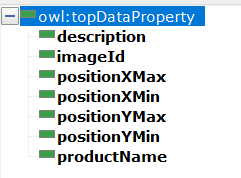
\includegraphics[width=0.7\linewidth]{images/dataproperties}
	\caption[Zbiór wszystkich właściwości istniejących obiektów]{}
	\label{fig:dataproperties}
\end{figure}



Brak dostosowania odpowiedniej klasy na podstawie tych danych spowodowałby brak danych wyjściowych z przeprowadzonego wnioskowania. Byłoby to spowodowane nierozpoznaniem klasy produktu, która jest niezbędna przy przetwarzaniu indywiduów. W tym celu stworzono regułę SWRL, która na podstawie nazwy produktu - czyli wyniku klasyfikacji - przypisuje odpowiednią klasę ontologii. 

\begin{lstlisting}[caption={Przypisanie klasy do indywiduum.}]
 Rule: equal(?c, "cola"), productName(?p, ?c), 
		 Product(?p) -> CocaCola(?p)
\end{lstlisting}

Aby określić pozycję przedmiotu na zdjęciu zostały stworzone reguły, które sprawdzają odległość punktów X lub Y względem określonego minimum. W tym celu do klasy o nazwie Position stworzono indywidua - Bottom, Top, Left, Right, Middle. Przedstawiona poniżej reguła SWRL przestawia przyporządkowanie istniejącego indywidua pozycji.

\begin{lstlisting}[caption={Przypisanie pozycji LeftPosition do indywidua na podstawie właściwości XMin.}]
Rule: Product(?p), positionXMin(?p, ?pXMin), 
		 lessThan(?pXMin, 0.25) -> hasPosition(?p, LeftPosition)
\end{lstlisting}

Każdy z tworzonych indywiduów dodatkowo posiada właściwość imageId będącą identyfikatorem analizowanego obrazu. Jest ona niezbędna, ponieważ w przypadku wnioskowania mającego na celu sprawdzenie czy obok produktu znajduje się inny, niezgodny, wówczas musielibyśmy rozróżnić już istniejące indywidua ontologii. W tym celu przy sprawdzeniu odległości dwóch podmiotów klasyfikacji względem sieci, reguła SWRL dodatkowo sprawdza, czy należą do tego samego obrazu.

\begin{lstlisting}[caption={Reguła sprawdzająca czy indywidua klas Pepsi oraz CocaColaZero znajdują się na tym samym obrazie}]
Rule: CocaColaZero(?cz), Pepsi(?p), imageId(?cz, ?czId), 
		 imageId(?p, ?pId), swrlb:equal(?pId, ?czId) 
		 -> Invalid(?cz), Invalid(?p), 
		 hasPositionMessage(?p, CocaColaOnTheSameScreenWithPepsi),
		 hasPositionMessage(?cz, CocaColaOnTheSameScreenWithPepsi)
\end{lstlisting}

W przypadku sklasyfikowania przedmiotu na obrazie jako produkt chemiczny stworzono regułę, która sprawdza czy jest on z dala od napojów. Miałaby ona między innymi wyeliminować szkodliwe ułożenie chemii, która mogłaby mieć wpływ na napoje. W tym celu reguła sprawdzi odległość pomiędzy analizowanymi produktami oraz przynależność do zdjęcia.

\begin{lstlisting}[caption={Reguła sprawdzająca bliską odległość środka chemicznego od napoju}]
Rule: Chemicals(?c), Drinks(?d), imageId(?c, ?cId), 
		 imageId(?d, ?dId), swrlb:equal(?dId, ?cId), 
		 positionXMin(?d, ?dPosX), positionXMax(?c, ?cPosX),
		 subtract(?posX, ?dPosX, ?cPosX), lessThan(?posX, 0.7) 
		 -> Invalid(?c), Invalid(?d),
		  isCloseToChemicals(?d, ChemicalCloseToProduct), 
		  isCloseToProduct(?c, ChemicalCloseToProduct)
\end{lstlisting}
\item \textbf{Generowanie raportów} - każdorazowe wywołanie mechanizmów wnioskujących powoduje zapisanie nowo dodanych indywiduów. Dzięki tej system ProductScanner posiada możliwość generowania raportów na podstawie zgromadzonych danych w ontologii. W tym celu użyto języka SPARQL, który pozwolił na stworzenie zpaytań wywoływanych z interfejsu JENA. Przykład sposobu otrzymywania danych niezbednych do wygenerowania raportów został przedstawiony w listingu \ref{reportGeneration}

\begin{lstlisting}[caption={Wykonywania zapytania SPARQL na istniejącej bazie wiedzy.}, label={reportGeneration}]
private Map<String, Integer> readIndividualCounter(String query)
{
	Query query = QueryFactory.create(query);
	QueryExecution qexec = SparqlDLExecutionFactory
		.create(query, _model);
	HashMap<String, Integer> result = new HashMap<>();
	ResultSet resultSet = qexec.execSelect();
	while (resultSet.hasNext()) {
		QuerySolution soln = resultSet.nextSolution();
		System.out.println(soln.toString());
		String key =soln.getResource("name").toString();
		String name = EscapeReasonerResult(key);
		String valueString = soln.getLiteral("total").toString();
		String escapedValue = GetNumberFromResult(valueString);
		result.put(name, Integer.parseInt(escapedValue));
	}
	return result;
}
\end{lstlisting}

Przedstawiona metoda wymaga przekazania jako parametr funkcji zapytania SPARQL stworzonego wcześniej w programie. W tym przypadku wymaga, aby w otrzymanym wyniku znajdowały się właściwości "name" oraz "total". Metoda została użyta w celu wykonania zapytania zliczającego ilość indywiduów poszczególnych klas produktów. Dzięki temu użytkownik zna podział produktów wykrytych na zdjęciach. Zapytanie SPARQL przekazane do metody \ref{reportGeneration} zostało przedstawione w listingu \ref{sparqlCountProducts}.

Zmiana zachowania ciała metody wewnątrz pętli while umożliwi bardzo szybkie dostosowanie kolejnych zapytań. Dzięki temu było możliwe otrzymanie danych dotyczących ilości niepoprawnie ułożonych sklasyfikowancyh przedmiotów oraz o ogólnej ilości indywiduów klasy Product. W zapytaniu SPARQL została przedstawione wykorzystanie polecenia count. Jednak w przypadku otrzymania pojedyńczego wyniku, biblioteka JENA generowała wartość równą null. W tym celu zliczono ilość wszystkich indywiduuów oraz ich cech za pomocą wyfiltrowanych wyników z zapytania SPARQL, które zostało zaprezentowane na listingu \ref{countInvalidProducts}.

\begin{lstlisting}[caption={Zapytanie SPARQL zliczające ilość sklasyfikowanych indywiduów.}, label={sparqlCountProducts}]
SELECT ?y (count(?y) as ?total)
WHERE {
{	?x a ont:CocaCola. 
	?x rdf:type ?y. 
	?y rdfs:subClassOf ont:CocaCola} UNION 
{ 	?x a ont:Pepsi.   
	?x rdf:type ?y.  
	?y rdfs:subClassOf ont:Pepsi} UNION 
{	?x a ont:CocaColaZero.  
	?x rdf:type ?y. 
	?y rdfs:subClassOf ont:CocaColaZero} .
}
group by ?y
\end{lstlisting}


\begin{lstlisting}[caption={Zliczenie niepoprawnie ułożonych przedmiotów}, label={countInvalidProducts}]
SELECT (count(?individuals) as ?total)
WHERE {
?cls rdfs:subClassOf ont:Invalid.
?individuals a ?cls.
?individuals a ont:Product}
\end{lstlisting}




\end{itemize}